%--------Experimentación
%--------Daniel Ochoa John
%--------20/07/2014
\newcolumntype{L}[1]{>{\raggedright\let\newline\\\arraybackslash\hspace{0pt}}m{#1}}
\newcolumntype{C}[1]{>{\centering\let\newline\\\arraybackslash\hspace{0pt}}m{#1}}
\newcolumntype{R}[1]{>{\raggedleft\let\newline\\\arraybackslash\hspace{0pt}}m{#1}}

\chapter{Experimentación}
\label{cap:experimentacion}

En este capítulo se tratará el experimento realizado, ejecutado bajo todo el desarrollo tecnológico descrito en los Capítulos 3 y 4, que implica la manera de probar la hipótesis que este trabajo de tesis postula. En primer lugar, se describe el experimento realizado, considerando inputs, outputs y puntos de evaluación. Luego, se caracterizan los \textit{data\textit{set}} utilizados, describiendo su dominio y cuantificando su tamaño. Finalmente, se muestran los resultados obtenidos.

\section{Descripción del experimento}

En esta sección se describe el experimento que se ha realizado para cumplir con el objetivo general de este trabajo, que es probar que existe una mejora en la eficiencia de la recomendación al contar con un mecanismo de persistencia y reutilización de las comunidades detectadas al momento de recomendar contenido a los usuarios.

Para describir el experimento, es necesario mencionar que, en el flujo de datos propuesto por RBox, al momento de generar una recomendación es posible también obtener comunidades de usuarios con intereses similares (ver Figura \ref{fig:exp-im1}). El asunto tiene que ver con persistir la existencia de las comunidades y utilizarlas como un antecedente que haga más eficiente recomendaciones posteriores, por lo que el experimento buscará evaluar si persistir las comunidades detectadas en una primera recomendación acelera o no el proceso de recomendación en ejecuciones posteriores, sobre un sistema de recomendación generado con RBox.

\begin{figure}
  \centering
  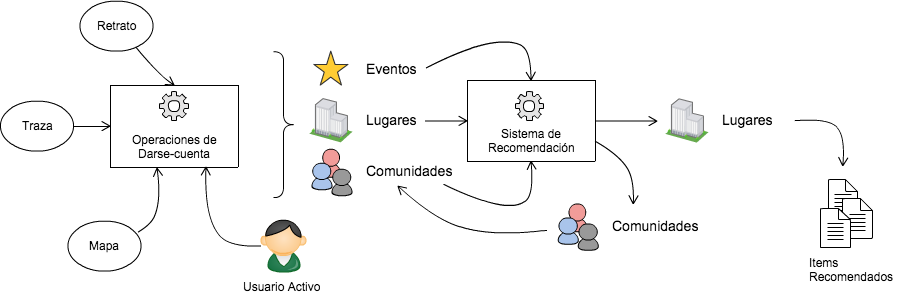
\includegraphics[scale=.6]{images/Figura5-1}
  \caption{\em Ciclo de recomendación en RBox.}
  \label{fig:exp-im1}
\end{figure}

Con este objetivo es que se ha generado un \textit{data\textit{set}} que será descrito en la sección siguiente. Sobre él se generará una recomendación de \textit{tags} considerando detección de comunidades, en dos escenarios: persistiendo comunidades detectadas y no persistiendo comunidades detectadas. La detección de comunidades será llevada a cabo mediante los distintos algoritmos que provee el servicio, ya descritos en el Capítulo 4. Luego, se comparan los tiempos de ejecución considerando ambos escenarios, para cada uno de los algoritmos de detección de comunidades.

\section{Caracterización de \textit{data\textit{set}}}

El \textit{data\textit{set}} que se ha utilizado para llevar a cabo el experimento ha sido obtenido a partir de la red social \textit{Twitter}. En concreto, se han generado un extractor de \textit{tweets} utilizando Ruby como lenguaje de programación. El extractor utiliza una gema llamada \textit{\textit{tweets}tream} para acceder a la Streaming API de \textit{Twitter}, permitiendo obtener el acceso a \textit{tweets} de índole público, en tiempo real. Cada uno de los \textit{tweets} es transformado a lógica 3-Ontology por el extractor y es persistido con la ayuda de un ORM\footnote{El mapeo objeto-relacional (en inglés \textit{Object Relational Mapping}, es una técnica que permite relacionar el diseño de clases de un diseño orientado a objetos, con un esquema de algún medio persistente.)} llamado Sequel\footnote{Fuentes y \textit{home} del proyecto en https://github.com/jeremyevans/sequel}.

El \textit{data\textit{set}} corresponde a una extracción dirigida de \textit{tweets}, orientado a la Copa Mundial de la Fifa Brasil 2014, para la que \textit{Twitter} ha promovido el uso de hash\textit{tags} particulares para cada país, como muestra la Tabla \ref{tab:exp-tab01}. Se ha hecho seguimiento a los comentarios que tengan que ver con los equipos sudamericanos que participan en la competición. La cuantificación de este \textit{data\textit{set}} se puede apreciar en la Tabla \ref{tab:exp-tab02}.  De cada uno de los \textit{tweets}, interesa saber de las siguientes interacciones:

\begin{enumerate}[I]
  \item \textbf{\textit{Mentioning}:} es el acto de referencia explícita, en un tweet, a un usuario. Denota un mensaje directo hacia otro usuario o una invitación a compartir una conversación respecto a un tema.
  \item \textbf{\textit{Tagging}:} es el acto de resaltar un concepto del mensaje utilizando un \textit{hashtag}. Generalmente, marca un tópico relevante que conlleva un interés particular del usuario, que motiva y fundamenta el contenido que ha compartido en la red social.
  \item \textbf{\textit{Replying}:} es el acto de replicar con un tweet la aseveración, comentario o mención de otro usuario.
\end{enumerate}

\begin{table}[H]
  \begin{center}
    \caption{Hash\textit{tags} particulares de cada país durante la copa mundial de la FIFA en \textit{Twitter}.}
    \label{tab:exp-tab01}
      \begin{tabular}{|L{4cm}|L{4cm}|}
        \hline
        \textbf{\textit{Hashtag}} & \textbf{País}\\ \hline
         \#CHI & Chile.\\ \hline
         \#BRA & Brasil.\\ \hline
         \#ARG & Argentina.\\ \hline
         \#COL & Colombia. \\ \hline
         \#ECU & Ecuador. \\ \hline
      \end{tabular}
  \end{center}
\end{table}

\begin{table}[H]
  \begin{center}
    \caption{Cuantificación del \textit{data\textit{set}} de la copa mundial de la FIFA.}
    \label{tab:exp-tab02}
      \begin{tabular}{|L{4cm}|L{4cm}|}
        \hline
        \textbf{Medida} & \textbf{Valor}\\ \hline
         \textit{Event} & 445.342\\ \hline
         \textit{Item} & 23.739\\ \hline
         \textit{User} & 91489\\ \hline
         \textit{Tweets} & 64.120\\ \hline
         \textit{Mentioning} & 92.519\\ \hline
         \textit{Tagging} & 349.577\\ \hline
         \textit{Replying} & 3.246\\ \hline
      \end{tabular}
  \end{center}
\end{table}

Como primer análisis, se considera el top 3 de usuarios que han compartido más \textit{tweets}, que incluyen menciones a otros usuarios (ver Tabla \ref{tab:exp-tab02}). Si se considera a estos usuarios, como activos, el grafo que representa sus interacciones se puede apreciar en las Figuras \ref{fig:exp-im2}, \ref{fig:exp-im3} y \ref{fig:exp-im4}, respectivamente. Si se realiza una detección de comunidades sobre el grafo de interacciones para estos usuarios, mediante, por ejemplo, del método \textit{Multilevel} (ver Capítulo 3), las comunidades detectadas pueden apreciarse en las Figuras \ref{fig:exp-im5}, \ref{fig:exp-im6} y \ref{fig:exp-im7}, respectivamente.

\begin{table}[H]
  \begin{center}
    \caption{Top 3 de usuarios con mas \textit{tweets} que consideran menciones a otros usuarios.}
    \label{tab:exp-tab02}
      \begin{tabular}{|L{4cm}|L{4cm}|}
        \hline
        \textbf{\textit{User} (Alias)} & \textbf{Nº de Menciones}\\ \hline
         539210296 (1) & 95\\ \hline
         2320149583 (2) & 85\\ \hline
         2463599637 (3)& 69\\ \hline
      \end{tabular}
  \end{center}
\end{table}

\begin{figure}
  \centering
  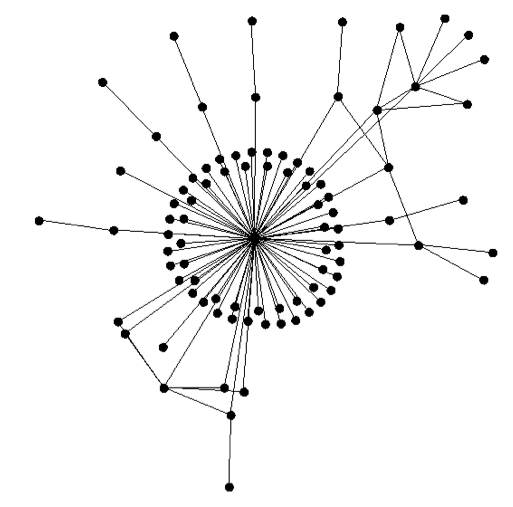
\includegraphics[scale=.7]{images/Figura5-2}
  \caption{\em Grafo de interacciones generado por el usuario 1.}
  \label{fig:exp-im2}
\end{figure}

\begin{figure}
  \centering
  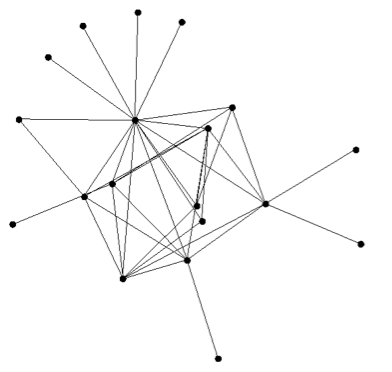
\includegraphics[scale=.7]{images/Figura5-3}
  \caption{\em Grafo de interacciones generado por el usuario 2.}
  \label{fig:exp-im3}
\end{figure}

\begin{figure}
  \centering
  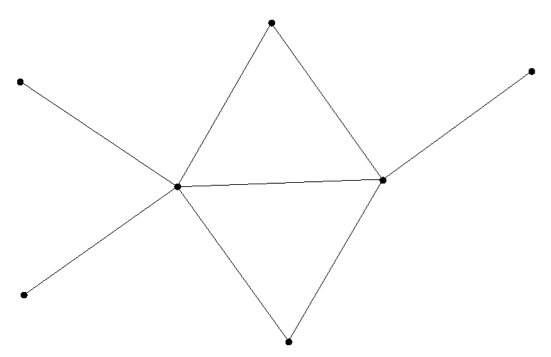
\includegraphics[scale=.7]{images/Figura5-4}
  \caption{\em Grafo de interacciones generado por el usuario 3.}
  \label{fig:exp-im4}
\end{figure}

\begin{figure}
  \centering
  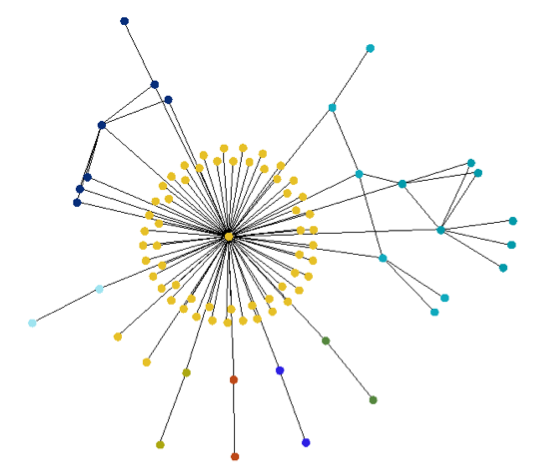
\includegraphics[scale=.7]{images/Figura5-5}
  \caption{\em Comunidades detectadas en base al grafo de interacciones generado por el usuario 1.}
  \label{fig:exp-im5}
\end{figure}

\begin{figure}
  \centering
  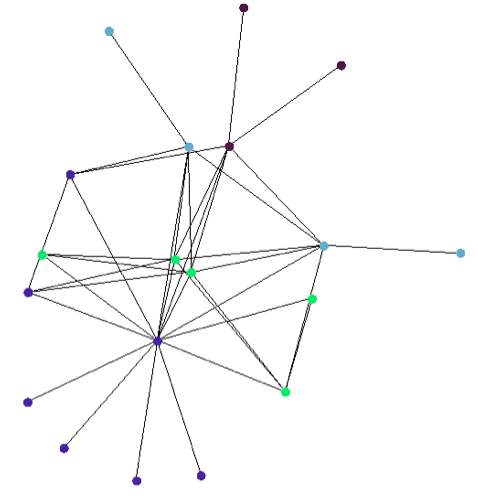
\includegraphics[scale=.7]{images/Figura5-6}
  \caption{\em Comunidades detectadas en base al grafo de interacciones generado por el usuario 2.}
  \label{fig:exp-im6}
\end{figure}

\begin{figure}
  \centering
  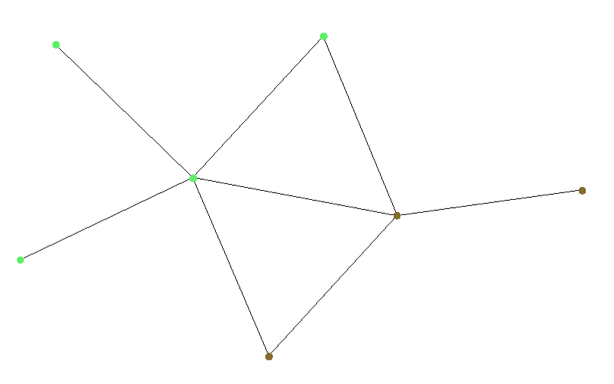
\includegraphics[scale=.7]{images/Figura5-7}
  \caption{\em Comunidades detectadas en base al grafo de interacciones generado por el usuario 3.}
  \label{fig:exp-im7}
\end{figure}

\section{Resultados}

Para experimentar con un proceso de recomendación utilizando comunidades, se ha implementado un algoritmo de recomendación de \textit{tags}, cuyo objetivo es retornar los top N \textit{tags} con mayor ocurrencia en una comunidad. Se han seleccionado dos usuarios (U), cuyos ids son 539210296 y 2320149583, para llevar a cabo la experimentación como usuarios activos. La Tabla \ref{tab:res-tab01} muestra los tiempos de ejecución requeridos para obtener la recomendación para los usuarios activos, dadas diez iteraciones (It), en las que se detectan comunidades, activando el primer nivel de \textit{community cache}, mediante distintos métodos (Mi): M1 (\textit{Multilevel}), M2 (LeadingEigenvector) y M3 (Infomap). La Tabla \ref{tab:res-tab02} muestra los tiempos de ejecución para un escenario similar, considerando detección de comunidades de manera forzada, al desactivar el primer nivel de \textit{community cache}.

Los dos escenarios recién mencionados consideran un ambiente sin comunidades en cada iteración, no obstante, un tercer escenario de pruebas es con comunidades existentes en el medio persistente, evaluando el segundo nivel de \textit{community cache}. En ese sentido la Tabla \ref{tab:res-tab03} muestra los tiempos de ejecución de aquel ejercicio.

Los resultados del primer escenario muestran que en la primera iteración el tiempo que se requiere para obtener la recomendación siempre es mayor que en las iteraciones posteriores. Esto es debido a que el proceso de recomendación antes de recomendar debe, en primera instancia, detectar y persistir las comunidades para el usuario activo.

En iteraciones posteriores el tiempo necesario para la recomendación se reduce debido a que, como la detección de comunidades no es forzada y dado que existen comunidades para ese usuario activo, debido al segundo nivel de \textit{community cache}, el \textit{framework} no requiere realizar el proceso de detección y persistencia. No obstante, los promedios de ejecución para todos los casos han aumentado en relación con el ejercicio anterior. Esto es debido a que, como se fuerza la detección de comunidades en cada iteración, el \textit{framework} detecta nuevamente las comunidades para el usuario activo, con la importante salvedad de que, gracias al segundo nivel de \textit{community cache}, no persiste aquellas que ya existen, eliminando duplicidad de comunidades.

Finalmente, el tercer escenario muestra que el tiempo de partida cuando no existen comunidades se ha reducido, en general, para ambos usuarios.  Esto último se confirma en la Tabla \ref{tab:res-tab04} donde se muestran los tiempos de ejecución promedio para los tres ejercicios ya mencionados.  Las Figuras \ref{fig:exp-im8} y \ref{fig:exp-im9} muestran respectivamente para cada usuario, el tiempo de ejecución promedio necesario para recomendar, considerando los tres experimentos. La reducción, en promedio, del tiempo necesario para obtener una recomendación para el usuario activo considerando el primer escenario y el último se ha reducido para todos los casos, incluso a pesar de que en el tercer escenario existen comprobaciones constantes de igualdad de comunidades debido a la \textit{community cache}.

En resumen, los escenarios considerados como prueba son:
\begin{enumerate}[I]
  \item Medio persistente sin comunidades al inicio del experimento. Primer nivel de \textit{community cache} activado. Medio persistente es reiniciado al momento de cambiar de usuario activo.
  \item Medio persistente sin comunidades al inicio del experimento. Primer nivel de \textit{community cache} desactivado. Medio persistente es reiniciado al momento de cambiar de usuario activo.
  \item Medio persistente sin comunidades al inicio del experimento. Primer nivel de \textit{community cache} desactivado. Medio persistente es compartido por todos los usuarios.
\end{enumerate}

\begin{table}[H]
  \begin{center}
    \caption{Tiempo en segundos que demora obtener una recomendación en el primer escenario.}
    \label{tab:res-tab01}
    \begin{tabular}{|l|l|l|l|l|l|l|}
      \hline
       & \multicolumn{3}{c|}{\textbf{U1}} & \multicolumn{3}{c|}{\textbf{U2}} \\ \hline
      \multicolumn{1}{|c|}{\textbf{It}} & \multicolumn{1}{c|}{\textbf{M1}} & \multicolumn{1}{c|}{\textbf{M2}} & \multicolumn{1}{c|}{\textbf{M3}} & \multicolumn{1}{c|}{\textbf{M1}} & \multicolumn{1}{c|}{\textbf{M2}} & \multicolumn{1}{c|}{\textbf{M3}} \\ \hline
      1 & 15,46 & 19,22 & 16,09 & 37,86 & 23,83 & 22,01 \\ \hline
      2 & 2,68 & 4,42 & 4,77 & 12,19 & 9,74 & 9,18 \\ \hline
      3 & 4,55 & 3,74 & 3,65 & 9,92 & 7,24 & 7,09 \\ \hline
      4 & 4,55 & 5,01 & 3,41 & 7,42 & 5,51 & 5,84 \\ \hline
      5 & 4,61 & 5,48 & 4,81 & 4,73 & 5,33 & 5,56 \\ \hline
      6 & 4,98 & 5,28 & 5,43 & 5,09 & 5,94 & 5,17 \\ \hline
      7 & 5,08 & 5,16 & 7,43 & 4,66 & 5,07 & 4,90 \\ \hline
      8 & 4,60 & 7,01 & 7,26 & 4,44 & 4,12 & 5,20 \\ \hline
      9 & 4,57 & 4,86 & 5,80 & 4,56 & 8,03 & 4,53 \\ \hline
      10 & 5,24 & 4,65 & 4,14 & 4,26 & 5,76 & 3,44 \\ \hline
    \end{tabular}
  \end{center}
\end{table}

\begin{table}[H]
  \begin{center}
    \caption{Tiempo en segundos que demora obtener una recomendación en el segundo escenario.}
    \label{tab:res-tab02}
    \begin{tabular}{|l|l|l|l|l|l|l|}
      \hline
       & \multicolumn{3}{c|}{\textbf{U1}} & \multicolumn{3}{c|}{\textbf{U2}} \\ \hline
      \multicolumn{1}{|c|}{\textbf{It}} & \multicolumn{1}{c|}{\textbf{M1}} & \multicolumn{1}{c|}{\textbf{M2}} & \multicolumn{1}{c|}{\textbf{M3}} & \multicolumn{1}{c|}{\textbf{M1}} & \multicolumn{1}{c|}{\textbf{M2}} & \multicolumn{1}{c|}{\textbf{M3}} \\ \hline
      1 & 9,05 & 8,72 & 8,98 & 26,60 & 23,05 & 15,78 \\ \hline
      2 & 5,23 & 4,26 & 4,87 & 13,00 & 10,70 & 10,26 \\ \hline
      3 & 5,83 & 4,63 & 4,67 & 9,52 & 8,07 & 8,14 \\ \hline
      4 & 5,01 & 5,56 & 4,90 & 7,82 & 7,02 & 6,68 \\ \hline
      5 & 4,60 & 5,03 & 5,92 & 8,90 & 6,42 & 5,92 \\ \hline
      6 & 5,02 & 4,98 & 5,93 & 6,70 & 5,30 & 5,81 \\ \hline
      7 & 5,17 & 5,94 & 4,87 & 5,42 & 5,03 & 5,82 \\ \hline
      8 & 4,89 & 5,32 & 5,58 & 5,73 & 5,30 & 5,51 \\ \hline
      9 & 5,39 & 4,85 & 5,54 & 5,30 & 5,07 & 4,71 \\ \hline
      10 & 5,66 & 5,23 & 4,64 & 5,42 & 5,53 & 4,82 \\ \hline
    \end{tabular}
  \end{center}
\end{table}

\begin{table}[H]
  \begin{center}
    \caption{Tiempo en segundos que demora obtener una recomendación en el tercer escenario.}
    \label{tab:res-tab03}
    \begin{tabular}{|l|l|l|l|l|l|l|}
      \hline
       & \multicolumn{3}{c|}{\textbf{U1}} & \multicolumn{3}{c|}{\textbf{U2}} \\ \hline
      \multicolumn{1}{|c|}{\textbf{It}} & \multicolumn{1}{c|}{\textbf{M1}} & \multicolumn{1}{c|}{\textbf{M2}} & \multicolumn{1}{c|}{\textbf{M3}} & \multicolumn{1}{c|}{\textbf{M1}} & \multicolumn{1}{c|}{\textbf{M2}} & \multicolumn{1}{c|}{\textbf{M3}} \\ \hline
      1 & 9,27 & 7,07 & 8,69 & 15,61 & 16,01 & 14,64 \\ \hline
      2 & 4,75 & 5,71 & 5,39 & 8,82 & 10,20 & 8,94 \\ \hline
      3 & 3,80 & 4,78 & 3,63 & 8,27 & 8,75 & 6,37 \\ \hline
      4 & 4,79 & 5,79 & 4,48 & 7,57 & 6,85 & 5,63 \\ \hline
      5 & 5,52 & 6,29 & 4,53 & 6,46 & 5,07 & 5,74 \\ \hline
      6 & 5,22 & 5,45 & 3,98 & 4,80 & 4,25 & 4,90 \\ \hline
      7 & 4,72 & 5,06 & 5,57 & 5,48 & 5,52 & 4,09 \\ \hline
      8 & 4,97 & 5,30 & 5,34 & 4,65 & 5,55 & 5,54 \\ \hline
      9 & 5,14 & 5,62 & 4,81 & 4,17 & 5,42 & 4,59 \\ \hline
      10 & 4,54 & 4,89 & 5,24 & 5,93 & 5,12 & 5,32 \\ \hline
    \end{tabular}
  \end{center}
\end{table}

\begin{table}[H]
  \begin{center}
    \caption{Tiempos promedio que demora la obtención de la recomendación detectando comunidades con los distintos escenarios (E).}
    \label{tab:res-tab04}
    \begin{tabular}{|l|l|l|l|l|l|l|}
    \hline
       & \multicolumn{3}{c|}{\textbf{U1}} & \multicolumn{3}{c|}{\textbf{U2}} \\ \hline
      \multicolumn{1}{|c|}{\textbf{It}} & \multicolumn{1}{c|}{\textbf{M1}} & \multicolumn{1}{c|}{\textbf{M2}} & \multicolumn{1}{c|}{\textbf{M3}} & \multicolumn{1}{c|}{\textbf{M1}} & \multicolumn{1}{c|}{\textbf{M2}} & \multicolumn{1}{c|}{\textbf{M3}} \\ \hline
      1 & 15,46 & 19,22 & 16,09 & 37,86 & 23,83 & 22,01 \\ \hline
      2 & 2,68 & 4,42 & 4,77 & 12,19 & 9,74 & 9,18 \\ \hline
      3 & 4,55 & 3,74 & 3,65 & 9,92 & 7,24 & 7,09 \\ \hline
      4 & 4,55 & 5,01 & 3,41 & 7,42 & 5,51 & 5,84 \\ \hline
      5 & 4,61 & 5,48 & 4,81 & 4,73 & 5,33 & 5,56 \\ \hline
      6 & 4,98 & 5,28 & 5,43 & 5,09 & 5,94 & 5,17 \\ \hline
      7 & 5,08 & 5,16 & 7,43 & 4,66 & 5,07 & 4,90 \\ \hline
      8 & 4,60 & 7,01 & 7,26 & 4,44 & 4,12 & 5,20 \\ \hline
      9 & 4,57 & 4,86 & 5,80 & 4,56 & 8,03 & 4,53 \\ \hline
      10 & 5,24 & 4,65 & 4,14 & 4,26 & 5,76 & 3,44 \\ \hline
    \end{tabular}
  \end{center}
\end{table}


\begin{figure}[H]
  \centering
  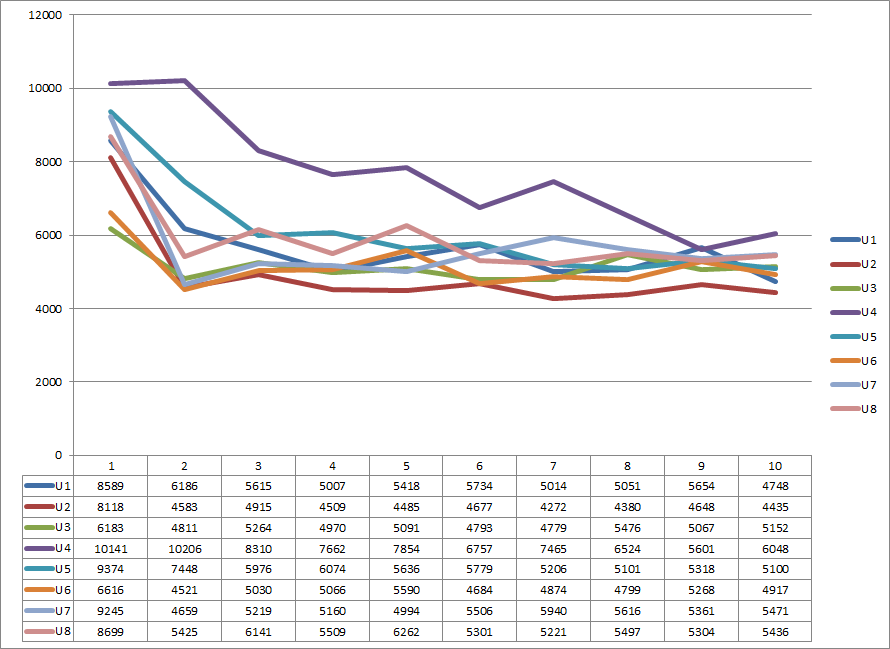
\includegraphics[scale=.7]{images/Figura5-8}
  \caption{\em Tiempos promedio para entregar una recomendación, en los distintos escenarios (E) de prueba, con el usuario 1 como activo.}
  \label{fig:exp-im8}
\end{figure}

\begin{figure}[H]
  \centering
  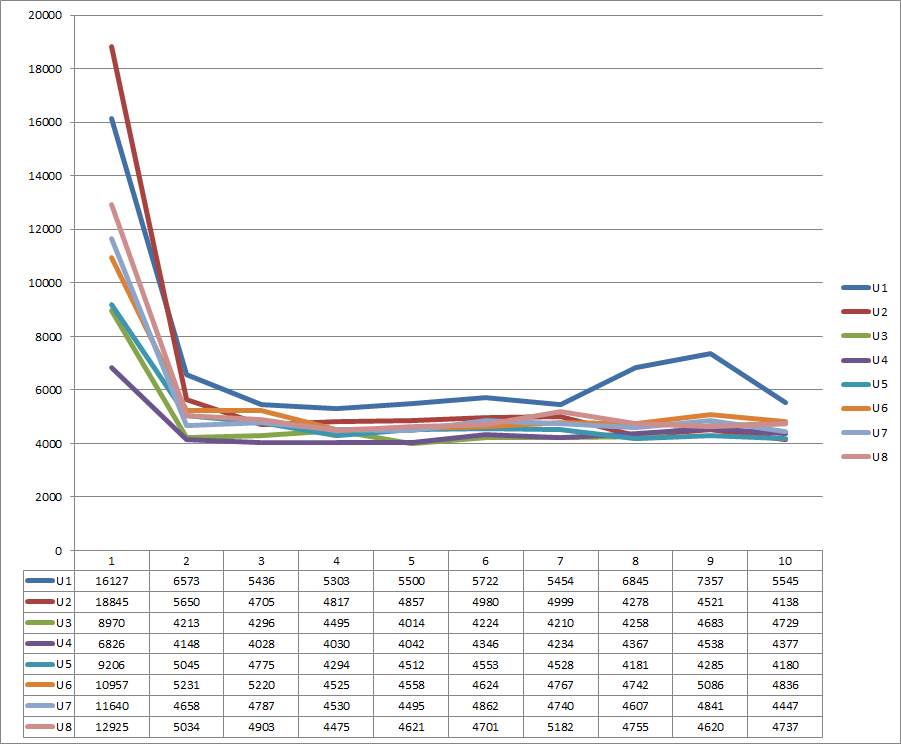
\includegraphics[scale=.7]{images/Figura5-9}
  \caption{\em Tiempos promedio para entregar una recomendación, en los distintos escenarios (E) de prueba, con el usuario 2 como activo.}
  \label{fig:exp-im9}
\end{figure}

\section{Resumen}

En este capítulo se ha descrito y presentado los resultados del experimento aplicado con el propósito de conseguir el objetivo general planteado en este trabajo de Tesis. En primer lugar, se ha descrito detalladamente el experimento realizado, con sus componentes y distintos escenarios. Luego, se ha caracterizado el \textit{data\textit{set}} utilizado para realizar las pruebas, describiendo el mecanismo de extracción, construcción, persistencia y cuantificación del tamaño de información contenida. Posteriormente, se han mostrado ejemplos de detección de comunidades utilizando el \textit{data\textit{set}} descrito. Finalmente, se han expuesto los resultados de la experimentación, logrando reducir el tiempo requerido para realizar una recomendación, mediante el uso del \textit{framework} y componentes descritos en los Capítulos 3 y 4.
